\documentclass[10pt,hyperref={citecolor=blue,anchorcolor=blue,urlcolor=blue,colorlinks=true,pdfpagelabels=true},dvipsnames]{beamer}
\usetheme{IITM}

% \includeonlyframes{cur}

\usepackage{mathtools}
\usepackage{accents}
\usepackage{graphicx}
\usepackage[english]{babel}
\usepackage{csquotes}
\usepackage{cancel}
\usepackage{soul}
\usepackage{appendixnumberbeamer}
\usepackage{cleveref}

\usepackage{qrcode}

\addbibresource{refs.bib}

% Custom Stuff %----------------------------------------------------------------------------------------------------------------------------------------------------------------
\newcommand{\vc}[1]{\underbar{$#1$}}
\newcommand{\mx}[1]{\mathbf{\underline{\underbar{$#1$}}}\,}

\newcommand{\uc}[1]{\underaccent{\tilde}{#1}}
\newcommand{\mc}[1]{\underaccent{\approx}{#1}}

\newcommand{\rtxt}[1]{\textcolor{red}{#1}}
\newcommand{\btxt}[1]{\textcolor{blue}{#1}}

\newcommand{\mathcolorbox}[2]{\colorbox{#1}{$\displaystyle #2$}}
\newcommand{\mhl}[1]{\colorbox{yellow}{$\displaystyle #1$}}

\renewcommand<>{\hl}[1]{\only#2{\beameroriginal{\hl}}{#1}}

\newcommand{\dd}{\mathrm{d}}

\usetikzlibrary{shadings,shapes.arrows,shapes.callouts,patterns,decorations.pathmorphing,
  decorations.markings,decorations.pathreplacing,shapes,arrows.meta}
\tikzset{
  invisible/.style={opacity=0},
  visible on/.style={alt={#1{}{invisible}}},
  alt/.code args={<#1>#2#3}{%
    \alt<#1>{\pgfkeysalso{#2}}{\pgfkeysalso{#3}} % \pgfkeysalso doesn't change the path
  },
}
\tikzset{
  highlight on/.style={alt={#1{fill=red!80!black,color=red!80!black}{fill=gray!30!white,color=gray!30!white}}},
}
\tikzset{
  nidbox/.style={fill=white, draw=red, thick, rounded corners=0.5mm, align=center}
}

\usetikzlibrary{tikzmark,calc,positioning}
\usepackage[markings,customcolors,beamer]{hf-tikz}
\hfsetfillcolor{yellow}
\hfsetbordercolor{none}

% Get rid of figure labels
\captionsetup{labelformat=empty,labelsep=none}
%----------------------------------------------------------------------------------------------------------------------------------------------------------------
\title[Abaqus4Joints]{An Abaqus-Matlab Tutorial for Jointed Systems}
\subtitle[ICJM Seminar]{International Committee on Jointed Structures Seminar Series}
\author[Balaji, N. N.]{Nidish Narayanaa Balaji}
\institute[AE, IITM]{Department of Aerospace Engineering, IIT Madras}
% ----------------------------------------------------------------------------------------------------------------------------------------------------------------

\begin{document}

\begin{frame}
  % \begin{beamercolorbox}[sep=0.3cm,ht=1.8em,wd=\paperwidth]{frametitle}
  %   \vbox{}\vskip-4ex%
  %   \strut\insertframetitle{\begin{tikzpicture}[remember picture,overlay]
  %       \node[anchor=north] at (current page.north) (A)
  %       {\includegraphics[height=1.75cm]{template/logo.png}};
  %     \end{tikzpicture}}\strut
  %   \vskip-0.5ex%				
  % \end{beamercolorbox}
  \titlepage
\end{frame}

\begin{frame}
  \frametitle{Table of Contents}
  \begin{columns}
    \centering
    \begin{column}{.5\textwidth}
      \tableofcontents{}
      \begin{figure}
        \centering
        \qrcode{https://nidish96.github.io/Abaqus4Joints/\#outline-container-orgfa25083}
        \caption{Detailed Instructions are \href{https://nidish96.github.io/Abaqus4Joints/\#outline-container-orgfa25083}{hosted through Github} in a repository named \href{https://github.com/Nidish96/Abaqus4Joints}{Nidish96/Abaqus4Joints} }
      \end{figure}
    \end{column}

    \begin{column}{.5\textwidth}
      \begin{block}{\centering Acknowledgements}
        \begin{itemize}
        \item Prof. Matthew Brake
        \item Dr. Justin Porter, Maeve Karpov
        \item Prof. Matt Allen
        \end{itemize}
      \end{block}
    \end{column}
  \end{columns}
\end{frame}

\section{Introduction}
\label{sec:introduction}

\begin{frame}
  \frametitle{The research needs of the joints community are quite unique and specific}
  \framesubtitle{\insertsectionnumber.~\insertsection}
  \begin{tikzpicture}[overlay,remember picture]
    \pgftransformshift{\pgfpointanchor{current page}{center}}

    \node[nidbox, text width=0.4\textwidth] at (-3.4521, 0.6389)
    {\textbf{The Generic Contact Problem}
      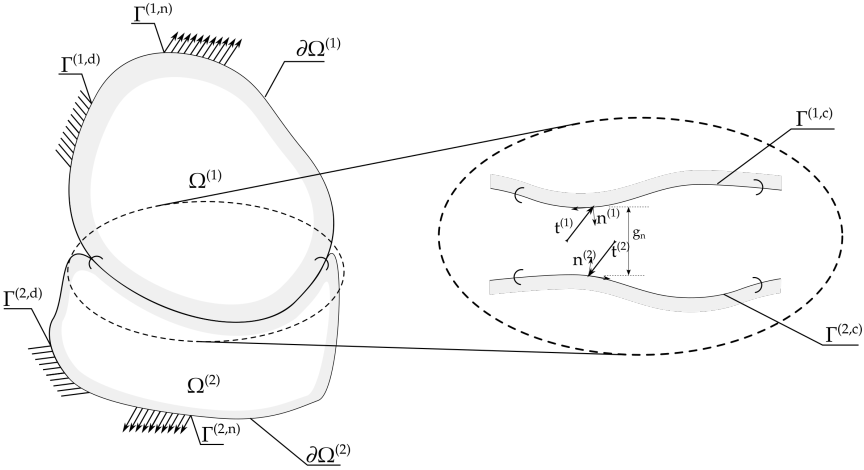
\includegraphics[width=\linewidth]{FIGS/contactprob}};

    \draw[red, very thick, rounded corners=0.5mm] (-0.4932, 2.4583) rectangle
    (6.1918, -3.0000);
    \node[align=center] at (2.8083, 2.2222) {Joints Benchmarks {\tiny
        \href{https://jointmechanics.org/index.php/Benchmarks}{(see
          jointmechanics.org)}}};
    \node[text width=0.15\textwidth] at (0.6027, 1.1528)
    {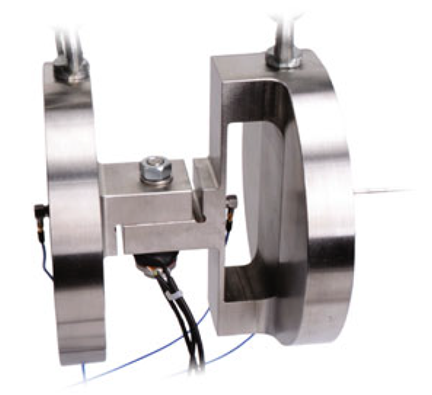
\includegraphics[width=\linewidth]{FIGS/roundres}};
    \node[text width=0.15\textwidth] at (2.4246, 1.2500)
    {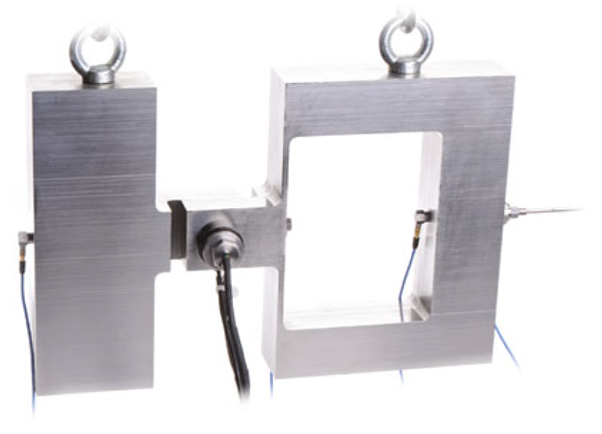
\includegraphics[width=\linewidth]{FIGS/gaulres}};
    \node[text width=0.15\textwidth] at (4.4383, 1.3055)
    {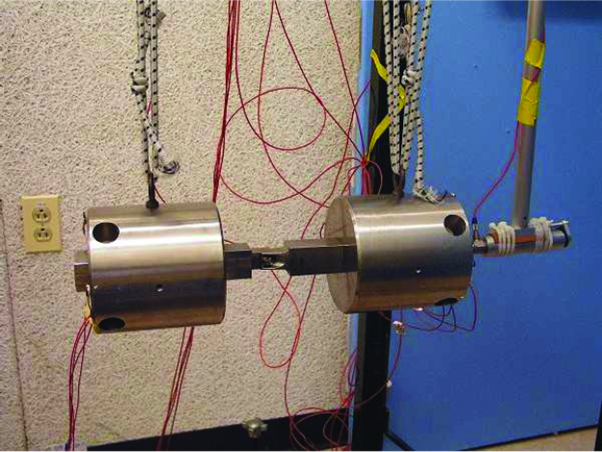
\includegraphics[width=\linewidth]{FIGS/dumbbellres}};

    \node[text width=0.4\textwidth] at (3.6987, -0.7639)
    {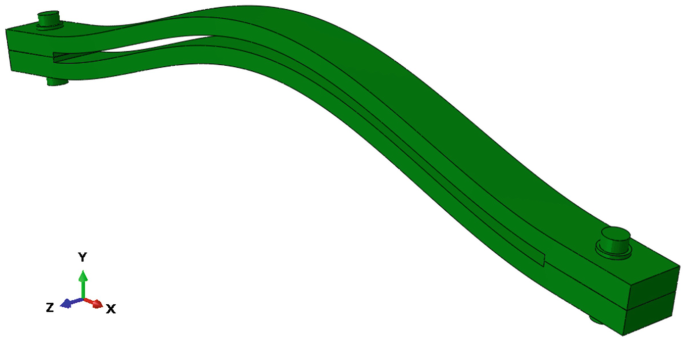
\includegraphics[width=\linewidth]{FIGS/s4bm}};
    \node[text width=0.4\textwidth] at (2.0137, -2.0138)
    {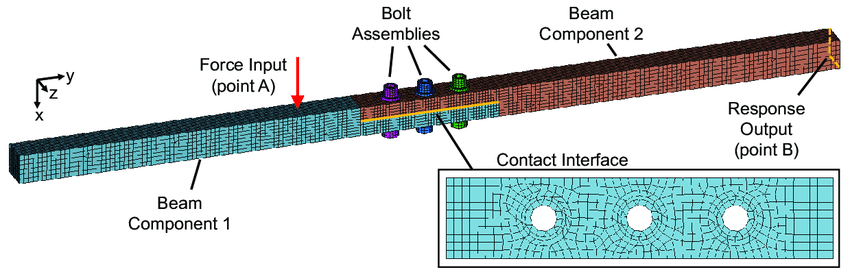
\includegraphics[width=\linewidth]{FIGS/brb}};

    \draw[red, very thick, rounded corners=0.5mm, fill=white, fill opacity=0.9,
    visible on=<2->] (-0.4932, 2.4583) rectangle (6.1918, -3.0000);
    \node[visible on=<2->, text width=0.5\textwidth, align=center] at
    (2.6164, -0.1528) {\rtxt{\textbf{Common theme}}: $\tikzmarkin<3>{a1}\text{Linear
        subcomponents}\tikzmarkend{a1}$ joined through a
      $\tikzmarkin<5->{a3}\text{non-linear contact interface}\tikzmarkend{a3}$
      undergoing $\tikzmarkin<4>{a2}\text{small deformation vibrations}\tikzmarkend{a2}$};

    \node[visible on=<3>, nidbox, text width=0.5\textwidth] at
    (2.5479, -2.8194) {\textbf{The HCB/CMS Methodology}
      
      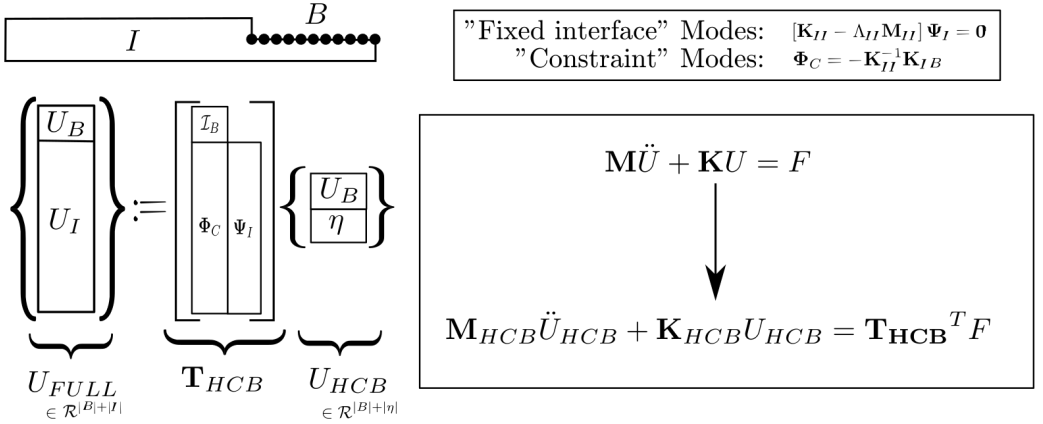
\includegraphics[width=\linewidth]{FIGS/hcb}
    };

    \node[visible on=<4>, nidbox, text width=0.5\textwidth] at
    (2.5479, -2.8194) {\textbf{Interface Virtual Element Representations}
      
      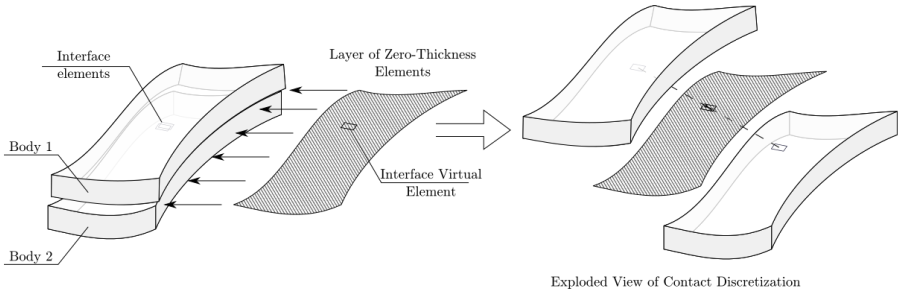
\includegraphics[width=\linewidth]{FIGS/ive}
    };

    \node[visible on=<5->, nidbox, text width=0.5\textwidth] at
    (2.5479, -2.8194) {\textbf{Interface Constitutive Modeling}
      
      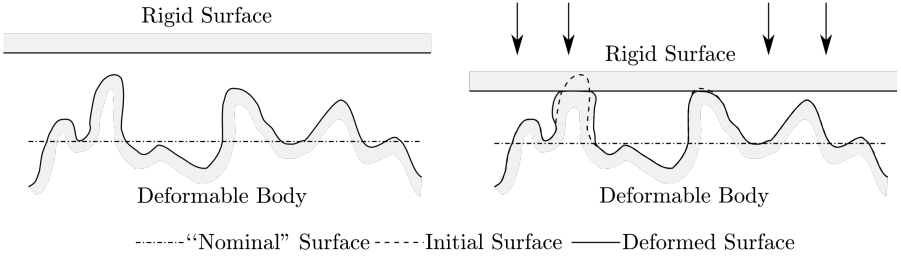
\includegraphics[width=\linewidth]{FIGS/roughc}
    };
  
    \node[visible on=<5->, text width=0.2\textwidth] at
    (-4.4383, -3.5833)
    {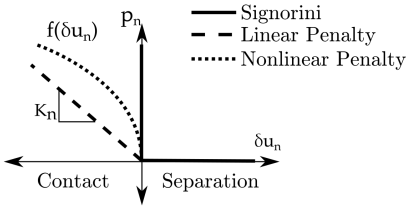
\includegraphics[width=\linewidth]{FIGS/normc}};
    \node[visible on=<5->, text width=0.2\textwidth] at
    (-2.0684, -2.9723)
    {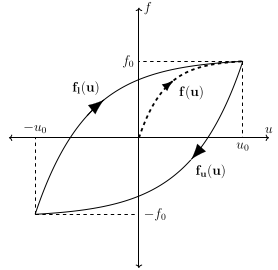
\includegraphics[width=\linewidth]{FIGS/tangc}};
    \node[visible on=<5->, text width=0.135\textwidth] at
    (-3.7260, -2.1944)
    {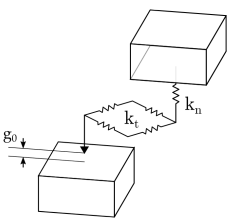
\includegraphics[width=\linewidth]{FIGS/contel}};      

    \node[visible on=<6->, nidbox, text width=0.43\textwidth] at
    (-3.3699, 0.4027) {\textbf{Nonlinear Responses}

      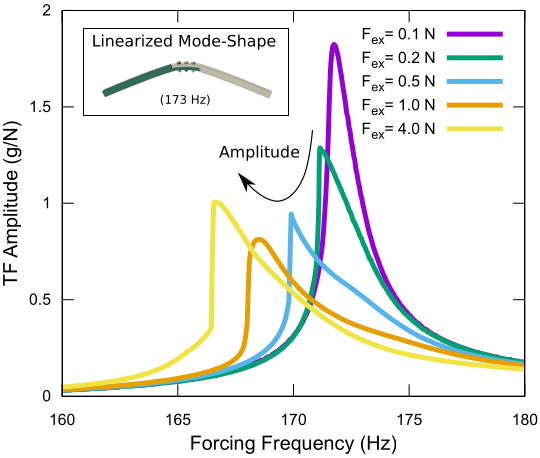
\includegraphics[width=0.8\linewidth]{FIGS/nlresp}
    };

    \node[visible on=<7->, nidbox, very thick, text
    width=0.6\textwidth] at (2.2877, 2.0556) {\rtxt{\textbf{Goal}}: Off-Load
      as much as possible to \textbf{focus on joints}.};
  \end{tikzpicture}
\end{frame}

\section{Outline of the Steps}
\label{sec:outline-steps}

\begin{frame}
  \frametitle{An Overview of the Modeling Pipeline}
  \framesubtitle{\insertsectionnumber.\insertsection}
  \begin{figure}
    \centering
    \includegraphics<1-7>[width=0.9\linewidth]{FIGS/ovw}
  \end{figure}

  \begin{tikzpicture}[overlay,remember picture]
    \pgftransformshift{\pgfpointanchor{current page}{center}}

    \draw[fill opacity=0.9, visible on=<2-5>, fill=white, draw=none]
    (0.0000, 3.0972) rectangle (5.5753, -4.5278);

    \draw[fill opacity=0.9, visible on=<2-5>, fill=white, draw=none]
    (-5.2877, -1.8611) rectangle (-0.3014, -4.2500);
    \draw[fill opacity=0.9, visible on=<2-4>, fill=white, draw=none]
    (-2.7945, 0.2500) rectangle (-0.2877, -1.8889);
    \draw[fill opacity=0.9, visible on=<2-3>, fill=white, draw=none]
    (-5.2740, 0.2639) rectangle (-2.7671, -1.8611);
    
    \node[visible on=<2>, text width=0.5\textwidth] at (-2.5890,
    1.2917) {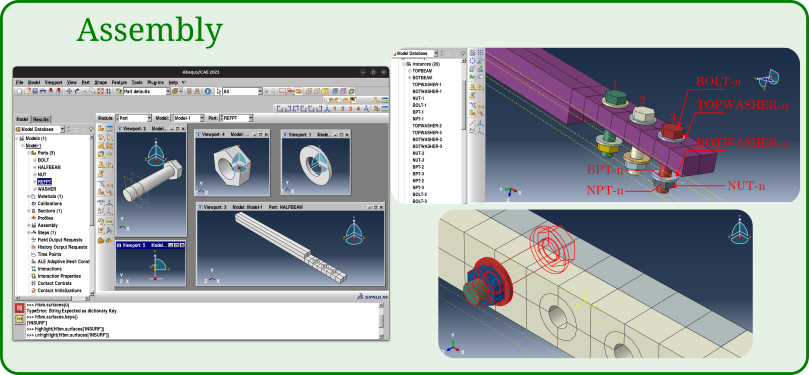
\includegraphics[width=\linewidth]{FIGS/1_Assembly}};
    \node[visible on=<3>, text width=0.25\textwidth] at (-4.0273,
    -0.7917) {\includegraphics[width=\linewidth]{FIGS/2_Constraints}};
    \node[visible on=<4>, text width=0.25\textwidth] at (-1.2603,
    -0.8750) {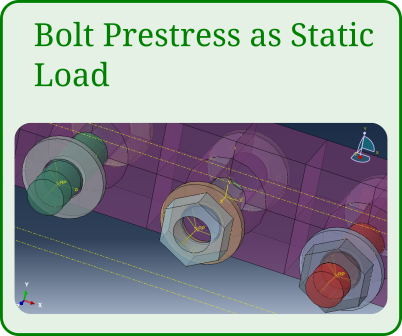
\includegraphics[width=\linewidth]{FIGS/3_BoltLoad}};
    \draw[-Latex, red, very thick, visible on=<4>] (-2.3288, -0.9861)
    -- (-2.6575, -1.3889);
    \draw[Latex-, red, very thick, visible on=<4>] (-1.3014, -1.3194)
    -- (-1.6301, -1.7222);
    \node[visible on=<4>, nidbox, text width=0.3\textwidth] at
    (2.6438, -0.7500) {\rtxt{\textbf{"Pull the Bolts, Push the Washers"}}};
    
    \node[visible on=<5>, text width=0.5\textwidth] at (-2.7123,
    -3.0833) {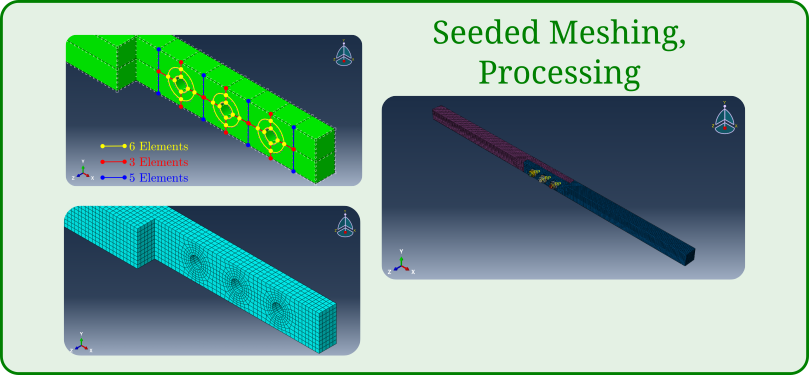
\includegraphics[width=\linewidth]{FIGS/4_Meshing}};


    \node[visible on=<6>, text width=0.5\textwidth] at (2.5205,
    -2.6528) {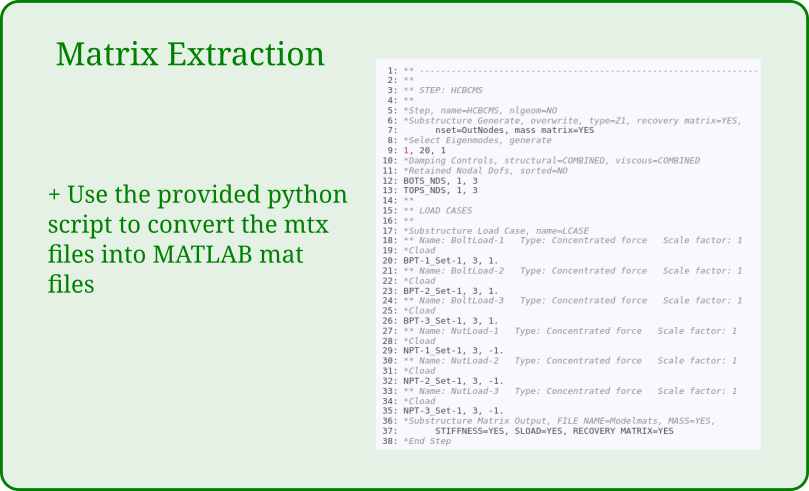
\includegraphics[width=\linewidth]{FIGS/5_matrixextract}};    
  \end{tikzpicture}
\end{frame}

\subsection{Relative Coordinates Pipeline}

\begin{frame}[label=cur]
  \frametitle{\insertsectionnumber.\insertsubsectionnumber.~\insertsubsection}
  \framesubtitle{\insertsection}
  \begin{itemize}
  \item Suppose that $\vc{u}_T, \vc{u}_B, \vc{u}_I$ are the vectors of top, bottom, and internal nodal DoFs. 
  \item Then the governing equations look like:
    \small
    \begin{align*}
      \begin{bmatrix} \mx{M}_{TT} & \mx{M}_{TB} & \mx{M}_{TI}\\
         & \mx{M}_{BB} & \mx{M}_{BI}\\
        \text{sym} &  & \mx{M}_{II} \end{bmatrix}
      \begin{bmatrix} \vc{\ddot{u}}_T\\ \ddot{\vc{u}}_B\\ \ddot{\vc{u}}_I \end{bmatrix}
      +
      \begin{bmatrix} \mx{K}_{TT} & \mx{K}_{TB} & \mx{K}_{TI}\\
         & \mx{K}_{BB} & \mx{K}_{BI}\\
        \text{sym} &  & \mx{K}_{II} \end{bmatrix}
      \begin{bmatrix} \vc{u}_T\\ \vc{u}_B\\ \vc{u}_I \end{bmatrix} +
      \begin{bmatrix} \tikzmarkin<3>{b1} \vc{F}^{(c)}_T\\ \vc{F}^{(c)}_B\\ \vc{0} \tikzmarkend{b1} \end{bmatrix} = \vc{F}_{e}(t)
    \end{align*}
  \item<2-> Under the relative coordinate transformation,
    \begin{align*}
      \begin{bmatrix} \vc{u}_T\\ \vc{u}_B\\ \vc{u}_I \end{bmatrix} =
      \begin{bmatrix} \mx{I}_T & \mx{I}_T & \mx{0}\\
        \mx{0} & \mx{I}_T & \mx{0}\\
        \mx{0} & \mx{0} & \mx{I}_I \end{bmatrix}
      \begin{bmatrix} \Delta \vc{u}\\ \vc{u}_B\\ \vc{u}_I \end{bmatrix},\qquad
      \Delta \vc{u} = \vc{u}_T-\vc{u}_B.
    \end{align*}
  \end{itemize}

  \begin{tikzpicture}[overlay,remember picture]
    \pgftransformshift{\pgfpointanchor{current page}{center}}

    \draw[visible on=<2->, red, -Latex] (-2.9178, -1.3334) .. controls
    (-2.4795, -0.5278) and (-1.5616, -0.8056) .. (-1.3288, -0.5417);

    \node[visible on=<3->, text width=\textwidth] at (-0.2329,
    -2.3889) {
      \begin{block}{\centering Transformed Equations of Motion}
        \scriptsize
        \begin{align*}
          \begin{bmatrix} \mx{M}_{TT} & \mx{M}_{TT}+\mx{M}_{TB} &
                                                                  \mx{M}_{TI}\\\\
                                      & \mx{M}_{TT}+\mx{M}_{BB}+ &
                                                                   \mx{M}_{TI}+\mx{M}_{BI}\\
            & \mx{M}_{TB}+\mx{M}_{TB}^T\\
            \text{sym} & & \mx{M}_{II} \end{bmatrix}
          \begin{bmatrix} \ddot{\vc{u}}_T\\\\ \tikzmarkin<4>{b3}\ddot{\vc{u}}_B\\\\
            \ddot{\vc{u}}_I\tikzmarkend{b3} \end{bmatrix}
          +
          \begin{bmatrix} &&\\\\ & \overline{K} & \\\\ && \end{bmatrix}
          \begin{bmatrix} \vc{u}_T\\\\ \tikzmarkin<4>{b4}\vc{u}_B\\\\
            \vc{u}_I\tikzmarkend{b4} \end{bmatrix}
          +
          \begin{bmatrix} \tikzmarkin<3>{b2} \vc{F}^{(c)}_T\\\\ \vc{0}\\\\
            \vc{0} \tikzmarkend{b2} \end{bmatrix}
          = \vc{F}_e(t).
        \end{align*}
      \end{block}
    };

    \node[visible on=<5->, text width=0.75\textwidth, nidbox] at
    (0, 0) {It is clearly advantageous (when possible) to
      use the relative coordinate transformation as early as possible
      in the CMS process.

      \rtxt{\textbf{Thankfully, this is possible fully in Abaqus itself!}}
    };
  \end{tikzpicture}
\end{frame}

\begin{frame}[label=cur]
  \frametitle{\insertsectionnumber.\insertsubsectionnumber.~\insertsubsection}
  \framesubtitle{\insertsection}

  \begin{itemize}
  \item By adding \ul{Reference Points} to the model at the location of the interfacial nodes, we can create \rtxt{\textbf{slave nodes whos DoF will be the relative DoF of the corresponding nodes on the interface}}.
  \item This can be done quite easily with Python scripting (the website has a script for the BRB which can be adapted to arbitrary contexts). 
  \end{itemize}
  \begin{figure}
    \centering
    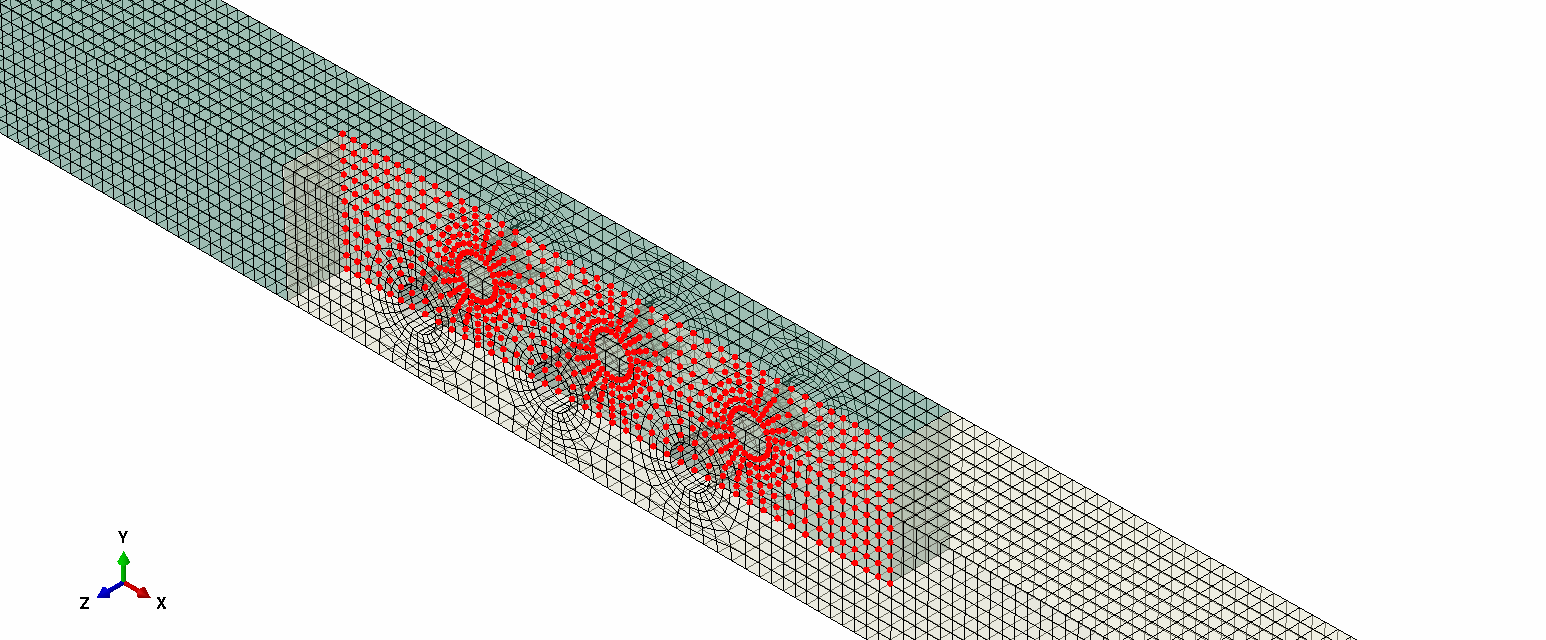
\includegraphics[width=0.8\linewidth]{FIGS/relcs}
  \end{figure}

  \begin{tikzpicture}[overlay,remember picture]
    \pgftransformshift{\pgfpointanchor{current page}{center}}

    \node[text width=0.4\textwidth] at (2.9178, -0.6389) {
      \begin{itemize}
      \item We can enforce the master-slave relationship using \emph{Equation Constraints}. 
      \end{itemize}
    };

    \node[visible on=<2->, nidbox, text width=0.8\textwidth] at
    (0, 0) {\textbf{...And this is what it looks like on ABAQUS.}

      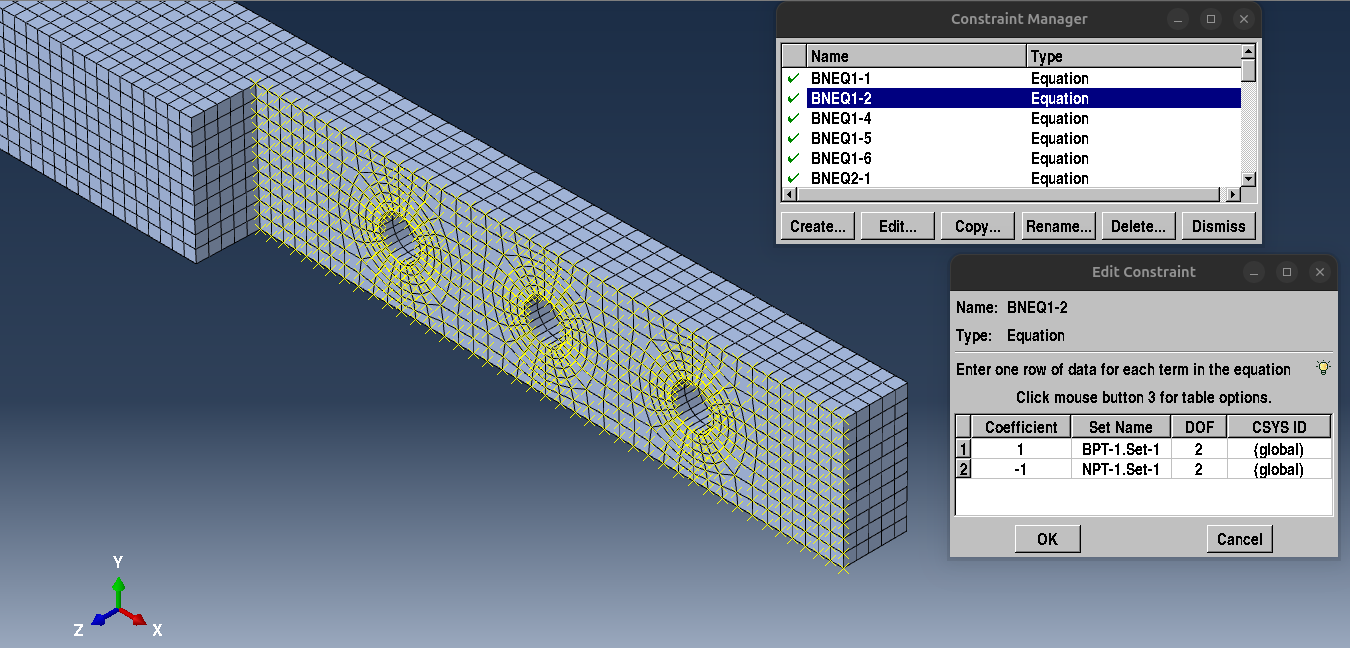
\includegraphics[width=\linewidth]{FIGS/rcs_pic}};

    \node[visible on=<3->, nidbox, text width=0.25\textwidth] at
    (-3.9178, -1.9444)
    {\textbf{.inp File Entries}:
      
      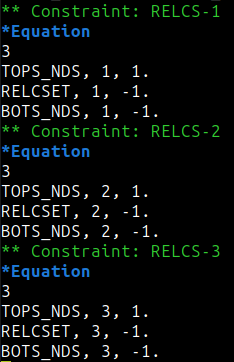
\includegraphics[width=0.9\linewidth]{FIGS/rcsinp}};

    \draw[-Latex, red, very thick] (0.2740, -1.9) -- (-2.4658,
    -1.9);
    \node[visible on=<3->, nidbox] at (0.6712, -1.9444) {$
      \vc{u}_{TOP} - \mhl{\vc{u}_{rel}} - \vc{u}_{BOT} = \vc{0} $};
  \end{tikzpicture}
\end{frame}

\section{Nonlinear Analysis in MATLAB}

\begin{frame}
  \frametitle{Nonlinear Analysis in Under 100 Lines of MATLAB Code!}
  \framesubtitle{\insertsectionnumber.~\insertsection}
  
\end{frame}

\section{Outro and Recommendations}
\label{sec:outro}

\begin{frame}
  \frametitle{\insertsectionnumber.~\insertsection}
  \begin{itemize}
  \item When we're interested in working on friction modeling at the interfacial level, it makes sense to off-load everything else to a software. 
  \item \hl{Try to think of ways to utilize the ABAQUS solvers as much as possible (for CMS modal analysis, etc.)}.
  \end{itemize}
  \begin{block}{\centering Some Drawbacks of this Pipeline}
    \begin{itemize}
    \item Applicability is \textbf{strictly restricted to small displacement contact}. 
    \item Geometrical Nonlinearities can't be present. If so, try an ICE fitting coupled with the relative coordinates approach.
    \end{itemize}
  \end{block}
\end{frame}

\begin{frame}
  \frametitle{\centering Thank You!}
  
  \begin{figure}
    \centering
    \qrcode{https://nidish96.github.io/Abaqus4Joints/\#outline-container-orgfa25083}
    \caption{\centering All the detailed instructions are \href{https://nidish96.github.io/Abaqus4Joints/\#outline-container-orgfa25083}{hosted through Github} in a repository named \href{https://github.com/Nidish96/Abaqus4Joints}{Nidish96/Abaqus4Joints} }    
  \end{figure}

  \centering
  Comments, suggestions and contributions welcome!\\
  Please email me at \href{mailto:nidish@iitm.ac.in}{nidish@iitm.ac.in}.  
\end{frame}

\begin{frame}[allowframebreaks]
  \frametitle{References}
  \renewcommand*{\bibfont}{\tiny}
  \vspace{-0.25cm}
  \printbibliography
\end{frame}

\end{document}

%%% Local Variables:
%%% mode: LaTeX
%%% TeX-master: t
%%% End:
